\subsection*{Robotic Arm Interface}
Although not as complete as the navigation interface, an interface has also been developed to allow for the use of the ROS arm\_navigation~\cite{RosArmNavWeb} stack. The {\it RosSim} node once again strives to allow for auto-discovery of the robot and thus eliminate the need for hand-generated configuration files. In the case of the arm\_navigation stack, a Unified Robot Description Format (URDF) file that describes the arm must be created as well as various launch files. 

Under USARSim, a robotic arm is composed of individual static meshes that are attached to one another via  links known as {\it actuators}. Each actuator has its own coordinate frame. Figure~\ref{Fig:KR60Anotated} depicts a Kuka KR60 robot that has been modeled in USARSim. The position and orientation of each actuator's coordinate frame is controlled by convention. Actuators must rotate (rotatory joints) or expand/contract (prismatic joints) about the z-axis. The x-axis must point towards the next joint in the kinematic chain. The location of the axis origin is constrained such that rotation/expansion occurs around $z=0$ and the x-axis passes through the origin of the next frame in the kinematic chain. The {\it RosSim} node automatically builds the transform tree for the various actuator coordinate frames by reading the USARSim {\it Conf} and {\it Geo} messages. The transform tree for the KR60 robot is depicted in Figure~\ref{Fig:KR60TF}. This transform is published and made available to any other ROS node.

When a new robotic arm is used for the first time, the {\it usar\_urdf} node of the {\it USARSim} ROS package must be run. This node accepts the same parameters shown in Table~\ref{Table:USARSimNode} in order to determine the robot to be created and then performs the following actions:
\begin{enumerate}
\item The node creates the robot model inside the simulated world in order to be able to read the USARSim  {\it Conf} and {\it Geo} messages.
\item From these messages, the node composes the transform tree with a transform for each joint in the robotic arm. Information on maximum and minimum rotations of joints and maximum joint velocities and torques is also maintained.
\item The node auto-generates an URDF file that contains all of the joint and link information that defines the robot arm. Rather than exact depictions of the robot's visual form, the URDF file contains simple cylinders to represent each link.
\end{enumerate}

\begin{figure}[t!]
\centering
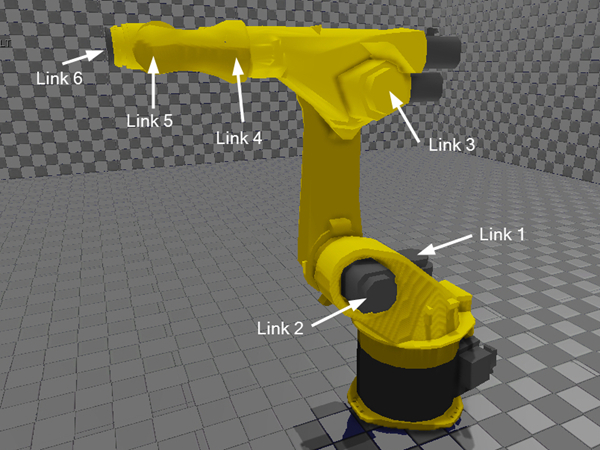
\includegraphics[width=8cm]{Figures/Robots/KR60Profile.jpg}
\caption{Location of joint axes in USARSim model of Kuka KR60 6 degree-of-freedom robot arm as depicted in USARSim.}
\label{Fig:KR60Anotated}
\end{figure}

\begin{figure}[t!]
\centering
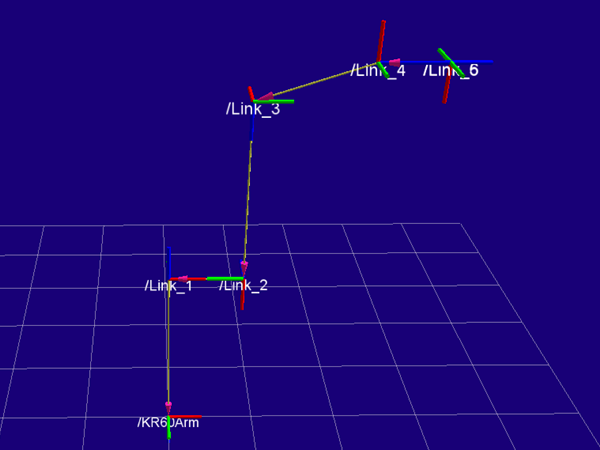
\includegraphics[width=8cm]{Figures/ROS/rviz1.png}
\caption{Depiction of joint axes from TF topic in ROS for 6 degree-of-freedom Kuka KR60 robot arm.}
\label{Fig:KR60TF}
\end{figure}

This URDF file may now be utilized by the arm\_naviation's {\it Planning Description Configuration Wizard} in order to generate a stack that contains specific launch files that will be used in arm planning.